本章围绕 LeRobot 在线推理循环中的三个主要阶段展开：
感知阶段负责采集两路相机图像和机械臂关节状态，推理阶段负责 ACT 策略前向计算，
执行阶段负责将动作通过舵机总线下发到 SO-101 follower。
三者虽然在 Python 主循环中串行出现，但其底层开销来源并不相同：
摄像头路径主要经过 OpenCV/V4L2 和用户态图像解码，
推理路径主要受 ARM CPU 上 PyTorch 算子计算限制，
舵机路径则受半双工串口总线和 SCServo 协议约束。

\subsection{感知阶段性能剖析}\label{sec:perception}

感知阶段对应主循环中的 \texttt{robot.get\_observation()}。
在本文的 SO-101 实验配置中，一次 observation 由两类数据组成：
两路 OpenCV 摄像头图像，以及一个 follower 机械臂的 6 个舵机当前位置。
其中两路摄像头分别为 \texttt{handeye} 和 \texttt{fixed}，分辨率均为
640$\times$360；舵机状态来自 6 个 STS3215 舵机的
\texttt{Present\_Position} 寄存器。

从代码结构看，SO-101 follower 的 \texttt{get\_observation()} 先通过
\texttt{self.bus.sync\_read("Present\_Position")} 同步读取 6 个舵机位置，
随后遍历 \texttt{self.cameras}，对每路相机调用
\texttt{cam.async\_read(timeout\_ms=3000)} 取得图像。
这意味着 obs 阶段并不是单一 I/O，而是“舵机同步读 + 两路相机异步取帧”的组合。
舵机读取与执行阶段的 \texttt{sync\_write} 共用同一条
\texttt{/dev/ttyACM0} 半双工总线，协议和内核路径高度重合，
因此本节只点明其在 obs 中的位置，详细分析放在 \S\ref{sec:execution}。

\subsubsection{摄像头异步读取机制}

LeRobot 的 OpenCV 相机并不是在主线程里每次直接阻塞读取硬件帧。
每个 \texttt{OpenCVCamera} 对象内部维护一个后台读线程，线程函数为
\texttt{\_read\_loop()}。源码中它是一个以
\texttt{stop\_event} 为退出条件的循环：只要没有收到停止信号，就反复通过
OpenCV 同步读取摄像头，把最新图像放入 \texttt{latest\_frame}，再用
\texttt{new\_frame\_event.set()} 告诉主线程“新帧已经准备好”。
主线程中的 \texttt{async\_read()} 不再直接面对摄像头设备，
而是等待这个事件；事件到达后，它只需短暂获取 \texttt{frame\_lock}，
从 \texttt{latest\_frame} 取走最近一帧，然后通过
\texttt{new\_frame\_event.clear()} 复位事件标志，等待下一次更新。
这里不是两个线程互相通知：后台线程负责生产帧并设置事件，主线程负责等待事件并清除事件。

\begin{figure}[htbp]
  \centering
  \begin{tikzpicture}[
    >=Stealth,
    lane/.style={rectangle, draw=gray!70, fill=gray!5, rounded corners=2pt,
      minimum width=2.6cm, minimum height=0.8cm, align=center, font=\small},
    proc/.style={rectangle, draw=blue!60, fill=blue!8, rounded corners=2pt,
      minimum width=2.9cm, minimum height=0.75cm, align=center, font=\footnotesize},
    shared/.style={rectangle, draw=orange!70, fill=orange!10, rounded corners=2pt,
      minimum width=2.9cm, minimum height=0.75cm, align=center, font=\footnotesize},
    note/.style={font=\scriptsize, text=gray!75}
  ]
    \node[lane] (bg) at (0, 2.1) {后台相机线程};
    \node[proc, right=0.8cm of bg] (read) {OpenCV 同步取帧\\V4L2 / MJPEG 解码};
    \node[shared, right=0.8cm of read] (cache) {更新 latest\_frame\\frame\_lock 保护};
    \node[proc, right=0.8cm of cache] (event) {set new\_frame\_event};

    \node[lane] (main) at (0, -0.35) {主线程 obs 阶段};
    \node[proc, right=0.8cm of main] (wait) {async\_read 等待事件};
    \node[shared, right=0.8cm of wait] (take) {读取 latest\_frame\\clear 事件标志};
    \node[proc, right=0.8cm of take] (return) {返回 observation 图像};

    \draw[->, thick, blue!65] (bg) -- (read);
    \draw[->, thick, blue!65] (read) -- (cache);
    \draw[->, thick, blue!65] (cache) -- (event);
    \draw[->, thick, red!65] (event.south) -- node[pos=0.55, right, note]{单向通知} (wait.north);
    \draw[->, thick, blue!65] (main) -- (wait);
    \draw[->, thick, blue!65] (wait) -- (take);
    \draw[->, thick, blue!65] (take) -- (return);
    \draw[->, thick, blue!65, rounded corners=8pt]
      (event.north) -- ++(0,0.55) -| node[pos=0.25, above, note]{未收到 stop\_event 时继续循环} (read.north);
    \draw[->, dashed, thick, gray!70, rounded corners=6pt]
      (take.north) -- ++(0,0.42) -| node[pos=0.32, below, note]{复位标志，不通知后台线程} (event.south);
  \end{tikzpicture}
  \caption{OpenCV 摄像头异步读取中的后台循环、单向事件通知与主线程取缓存关系}
  \label{fig:opencv-async-read}
\end{figure}

后台线程会调用 OpenCV 的读帧接口，从 V4L2 摄像头设备取出一帧，
并在用户态完成 MJPEG 解码和颜色格式整理。整理后的 RGB 图像被写入
\texttt{latest\_frame}，这个共享缓存由 \texttt{frame\_lock} 保护。
\texttt{new\_frame\_event} 只承担“帧已就绪”的单向通知作用；
主线程取走缓存帧后会复位事件标志，避免下一轮直接读到旧帧，
但这个复位动作不会反向唤醒或驱动后台相机线程。

因此，\texttt{async\_read()} 的“异步”含义是：摄像头硬件读取和 MJPEG 解码
提前在后台线程中进行，主线程在 obs 阶段只等待事件并读取最近一帧。
如果后台线程已经准备好图像，主线程很快返回；如果主线程跑得比相机帧率更快，
则会在等待新帧事件时阻塞。

\subsubsection{是否进入内核}

摄像头路径中有三类等待，需要区分其含义。

\begin{center}
\small
\begin{tabularx}{\textwidth}{>{\raggedright\arraybackslash}p{0.22\textwidth}
  >{\raggedright\arraybackslash}p{0.28\textwidth}
  >{\raggedright\arraybackslash}X}
  \toprule
  位置 & 是否可能进入内核 & 含义 \\
  \midrule
  主线程等新帧事件 & 可能进入内核 &
  线程同步等待。对应 \texttt{new\_frame\_event.wait()}，
  主线程等后台相机线程把新帧准备好 \\
  主线程取缓存帧 & 通常不进入内核 &
  短锁保护。对应 \texttt{frame\_lock}，
  只是在读写 \texttt{latest\_frame} 时避免两个线程同时改同一块缓存 \\
  OpenCV 后台线程取帧 & 会进入内核 &
  设备可读等待。后台线程通过 \texttt{select()} 等待 V4L2 摄像头有帧可取，
  随后再执行出队操作取得该帧 \\
  \bottomrule
\end{tabularx}
\end{center}

也就是说，主线程的 \texttt{async\_read()} 主要是在等 Python 线程同步事件；
真正深入 V4L2、USB 摄像头驱动和 videobuf2 队列的是后台读线程。
这也是为什么主线程观测耗时可能只有毫秒级，而摄像头后台线程的
\texttt{pselect6} 等待会接近 30 fps 的帧间隔。

\subsubsection{OpenCV 到内核的边界}

论文正文不展开完整源码栈，只保留性能分析需要的边界关系：
后台相机线程首先进入 OpenCV 的 \texttt{VideoCapture}，随后通过 glibc
发起 V4L2 相关系统调用，最终进入 Linux 的 V4L2、UVC 和 videobuf2 队列。

\begin{figure}[htbp]
  \centering
  \begin{tikzpicture}[
    >=Stealth,
    box/.style={rectangle, draw=blue!60, fill=blue!7, rounded corners=2pt,
      minimum width=2.65cm, minimum height=0.74cm, align=center, font=\scriptsize},
    waitbox/.style={rectangle, draw=orange!75, fill=orange!10, rounded corners=2pt,
      minimum width=2.65cm, minimum height=0.74cm, align=center, font=\scriptsize},
    kbox/.style={rectangle, draw=green!55!black, fill=green!7, rounded corners=2pt,
      minimum width=2.65cm, minimum height=0.74cm, align=center, font=\scriptsize},
    layer/.style={font=\scriptsize\bfseries, text=gray!80},
    note/.style={font=\scriptsize, text=gray!75}
  ]
    \node[layer] at (-1.45, 3.55) {Python / LeRobot};
    \node[box] (loop) at (0.95, 3.55) {后台相机线程\\\texttt{\_read\_loop()}};
    \node[box] (pyread) at (4.05, 3.55) {OpenCV Camera\\\texttt{read()}};
    \node[box] (tryioctl) at (7.15, 3.55) {\texttt{grab()}\\\texttt{tryIoctl(DQBUF)}};

    \node[note] at (2.35, 2.62) {无完成帧：等待设备可读};
    \node[note] at (7.15, 2.62) {已有完成帧：出队并解码};

    \node[layer] at (-1.45, 1.75) {glibc / syscall};
    \node[waitbox] (select) at (2.35, 1.75) {\texttt{select()}\\等待 fd 可读};
    \node[waitbox] (pselect) at (2.35, 0.65) {\texttt{pselect6}\\睡眠等待};
    \node[waitbox] (ioctl) at (7.15, 1.75) {\texttt{ioctl}\\\texttt{VIDIOC\_DQBUF}};

    \node[layer] at (-1.45, -0.45) {Linux kernel};
    \node[kbox] (v4l2) at (2.35, -0.45) {V4L2 / UVC\\设备驱动};
    \node[kbox] (wq) at (2.35, -1.55) {\texttt{done\_wq}\\等待队列};
    \node[kbox] (vb2) at (7.15, -0.45) {videobuf2\\完成队列};
    \node[box] (decode) at (7.15, -1.55) {\texttt{retrieve()}\\MJPEG 解码};

    \draw[->, thick, blue!65] (loop) -- (pyread);
    \draw[->, thick, blue!65] (pyread) -- (tryioctl);

    \draw[->, thick, orange!75, rounded corners=6pt]
      (tryioctl.south) -- ++(0,-0.38) -| node[pos=0.28, above, note]{无帧可取} (select.north);
    \draw[->, thick, orange!75] (select) -- (pselect);
    \draw[->, thick, orange!75] (pselect) -- (v4l2);
    \draw[->, thick, orange!75] (v4l2) -- node[right, note]{新帧完成} (wq);
    \node[note] at (2.35, -2.18) {唤醒后回到 DQBUF 重试};

    \draw[->, thick, green!55!black] (tryioctl) -- node[right, note]{已有完成帧} (ioctl);
    \draw[->, thick, green!55!black] (ioctl) -- (vb2);
    \draw[->, thick, green!55!black] (vb2) -- node[right, note]{buffer 元数据} (decode);

    \node[note] at (7.75, 3.03) {用户态};
    \draw[dashed, gray!55] (-0.10,2.28) -- (8.55,2.28);
    \node[note] at (7.60, 2.14) {系统调用边界};
  \end{tikzpicture}
  \caption{OpenCV 摄像头后台线程从用户态到 V4L2 内核队列的关键路径}
  \label{fig:opencv-v4l2-callstack}
\end{figure}

图~\ref{fig:opencv-v4l2-callstack} 中有两条需要区分的路径：
等待设备可读通常发生在 \texttt{select()} / \texttt{pselect6} 一类调用上；
真正取出已完成图像缓冲区时，OpenCV 使用 \texttt{VIDIOC\_DQBUF} 将一个已经由驱动填好的
V4L2 buffer 从完成队列中出队。

需要注意的是，\texttt{VIDIOC\_DQBUF} 并不是把整帧像素从内核重新拷贝一遍。
在当前 OpenCV V4L2 路径中，摄像头 buffer 通过 mmap 暴露给用户态；
出队操作主要返回 buffer 的编号、有效字节数和时间戳等元数据。
MJPEG 到 BGR 图像的解码仍然发生在用户态 OpenCV/libjpeg 中，
这部分才是 ARM CPU 上摄像头链路中更明显的计算开销。

完整的 OpenCV、glibc 和 Linux 内核源码级 CallStack 与参数说明，
不放在论文正文中展开，单独记录在
\texttt{robotdoc/摄像头相关/OpenCV到glibc到内核CallStack源码解析.md}。

\subsubsection{时间剖析}

在 30 fps 摄像头配置下，单路摄像头物理帧间隔约为 33.3 ms。
实测中，后台线程在 \texttt{pselect6} 或 V4L2 等待路径中阻塞约 23--32 ms，
符合摄像头帧率上限；MJPEG 解码仍在用户态 OpenCV/libjpeg 中完成，
在 ARM CPU 上属于摄像头链路的主要计算开销。
由于 LeRobot 采用后台预取，主线程 obs 阶段看到的是“取缓存帧”的时间，
而不是完整的摄像头端到端采集时间。

实测的逐层耗时分布与分层架构图见实验 06（摄像头感知层级耗时剖析，
\texttt{robotdoc/实验/06\_摄像头感知层级耗时剖析/}）\label{exp:06}。
该实验通过 ftrace 内核插桩和 Python \texttt{perf\_counter} 双层时间戳，
量化了从 \texttt{pselect6} 阻塞到 tensor 入模的层级耗时，
并区分了“端到端时延”与“主线程感知耗时”在异步预取下的差异。

\src{OpenCV视频流内部实现.md，OpenCV到glibc到内核CallStack源码解析.md，
pselect6最终结果.md，实验数据/06\_摄像头感知层级耗时剖析/README.md}

\subsection{推理阶段性能剖析}\label{sec:inference}

本节专门分析 SO-101 在线控制循环中的 ACT 策略推理阶段。
这里的“推理阶段”并不只是一次 \texttt{ACT.forward()}，
而是从 \texttt{predict\_action()} 收到 observation 开始，
经过动作缓存判断、必要时的观测预处理、ACT 模型前向、动作队列写入、
再到动作反归一化返回的完整路径。

当前实验配置中，ACT 的 \texttt{chunk\_size} 与
\texttt{n\_action\_steps} 均为 100，单次完整模型推理输出
\((B,\texttt{chunk\_size},\texttt{action\_dim})=(1,100,6)\) 的动作序列。
因此在线循环的大多数帧并不会重新执行模型前向，而是直接从
\texttt{\_action\_queue} 中取出上一次推理缓存的下一帧动作。
这一区别是理解第~\ref{sec:inference} 节所有时间数据的前提：
\texttt{chunk\_size} 主要是在时间上分摊单次 ACT 前向开销，
而不是让一次 ACT 前向本身变快。

\subsubsection{\texttt{select\_action} 与动作队列}

LeRobot 在 \texttt{predict\_action()} 外层先检查策略对象的动作队列。
如果 \texttt{\_action\_queue} 非空，主循环直接
\texttt{popleft()} 取出缓存动作，再通过 \texttt{postprocessor}
反归一化为真实舵机目标；这一帧会跳过图像 tensor 转换、
\texttt{preprocessor} 和 \texttt{ACT.forward()}。
只有当队列为空时，系统才会走完整推理路径：
把 numpy observation 转为 PyTorch Tensor，执行归一化预处理，
调用 \texttt{policy.select\_action()}，继而触发
\texttt{predict\_action\_chunk()} 和 \texttt{ACT.forward()}。
模型一次产生 100 帧归一化动作，写入队列后立即弹出第 0 帧返回；
后续 99 帧由队列快速路径逐帧取用。

\begin{figure}[htbp]
  \centering
  \begin{tikzpicture}[
    >=Stealth,
    node distance=0.7cm,
    box/.style={rectangle, draw=blue!60, fill=blue!7, rounded corners=2pt,
      minimum width=2.18cm, minimum height=0.70cm, align=center, font=\scriptsize},
    fast/.style={rectangle, draw=green!55!black, fill=green!8, rounded corners=2pt,
      minimum width=2.18cm, minimum height=0.70cm, align=center, font=\scriptsize},
    full/.style={rectangle, draw=orange!75, fill=orange!9, rounded corners=2pt,
      minimum width=2.18cm, minimum height=0.70cm, align=center, font=\scriptsize},
    note/.style={font=\scriptsize, text=gray!75, fill=white, inner sep=0.8pt}
  ]
    \node[box] (entry) at (0,0) {\texttt{predict\_action()}};
    \node[box] (check) at (2.55,0) {检查\\\texttt{\_action\_queue}};

    \node[fast] (pop) at (5.00,1.35) {\texttt{popleft()}\\缓存动作};
    \node[fast] (postfast) at (7.50,1.35) {\texttt{postprocessor}\\反归一化};
    \node[fast] (retfast) at (10.00,1.35) {返回\\当前动作};

    \node[full] (obs) at (5.00,-1.20) {numpy obs\\图像 / state};
    \node[full] (prep) at (7.50,-1.20) {tensor 化\\\texttt{preprocessor}};
    \node[full] (select) at (10.00,-1.20) {\texttt{policy}\\\texttt{select\_action()}};
    \node[full] (forward) at (10.00,-2.60) {action chunk\\\texttt{ACT.forward()}};
    \node[full] (queue) at (7.50,-2.60) {写入 100 帧队列\\弹出第 0 帧};
    \node[full] (postfull) at (5.00,-2.60) {\texttt{postprocessor}\\返回动作};

    \draw[->, thick, blue!65] (entry) -- (check);
    \draw[->, thick, green!55!black, rounded corners=6pt]
      (check.north) -- ++(0,1.65)
      -- ++(2.45,0)
      -- (pop.north);
    \node[note, text=green!45!black] at (3.75,2.17) {队列非空};
    \draw[->, thick, green!55!black] (pop) -- (postfast);
    \draw[->, thick, green!55!black] (postfast) -- (retfast);

    \draw[->, thick, orange!80, rounded corners=6pt]
      (check.south) -- ++(0,-0.28)
      -- ++(2.45,0)
      -- (obs.north);
    \node[note, text=orange!85!black] at (3.75,-0.86) {队列为空};
    \draw[->, thick, orange!80] (obs) -- (prep);
    \draw[->, thick, orange!80] (prep) -- (select);
    \draw[->, thick, orange!80] (select) -- (forward);
    \draw[->, thick, orange!80] (forward) -- (queue);
    \draw[->, thick, orange!80] (queue) -- (postfull);
  \end{tikzpicture}
  \caption{ACT 在线推理中动作队列快速路径与完整推理路径}
  \label{fig:act-select-action-queue}
\end{figure}

图~\ref{fig:act-select-action-queue} 说明了
\texttt{chunk\_size=100} 下的两种时间尺度：
队列非空帧只承担动作取队列和反归一化，属于轻量路径；
队列为空帧才承担完整 ACT 前向，属于重推理路径。
因此，按 episode 统计得到的 inference 占比，本质上是少数重推理帧
在 100 帧执行周期内被均摊后的结果。

\subsubsection{一次完整 ACT 推理的数据流}

队列为空时，\texttt{predict\_action()} 会先把原始 observation
整理成 ACT 可接受的 batch。两路相机图像从
\((H,W,C)\) 的 \texttt{uint8} numpy 数组转换为
\((1,3,360,640)\) 的 \texttt{float32} Tensor；
关节状态从 \((6,)\) 转为 \((1,6)\)。
随后 \texttt{preprocessor} 使用随 checkpoint 保存的训练集
mean/std 对图像、state 进行归一化。进入 \texttt{ACT.forward()}
后，推理态下不运行训练用 VAE encoder，而是使用全零 latent。

\begin{figure}[htbp]
  \centering
  \begin{tikzpicture}[
    >=Stealth,
    box/.style={rectangle, draw=blue!60, fill=blue!7, rounded corners=2pt,
      minimum width=2.25cm, minimum height=0.70cm, align=center, font=\scriptsize},
    prep/.style={rectangle, draw=orange!75, fill=orange!9, rounded corners=2pt,
      minimum width=2.25cm, minimum height=0.70cm, align=center, font=\scriptsize},
    model/.style={rectangle, draw=cyan!60!black, fill=cyan!8, rounded corners=2pt,
      minimum width=2.25cm, minimum height=0.70cm, align=center, font=\scriptsize},
    outbox/.style={rectangle, draw=green!55!black, fill=green!8, rounded corners=2pt,
      minimum width=2.25cm, minimum height=0.70cm, align=center, font=\scriptsize},
    note/.style={font=\scriptsize, text=gray!75, fill=white, inner sep=0.8pt}
  ]
    \node[box] (obs) at (0.0,3.05) {observation\\2 图像 + state};
    \node[prep] (tensor) at (2.55,3.05) {输入整理\\HWC $\to$ CHW};
    \node[prep] (norm) at (5.10,3.05) {mean/std\\归一化};

    \node[model] (resnet) at (1.25,1.45) {两路 ResNet18\\layer4 特征};
    \node[model] (visproj) at (4.00,1.45) {2D 位置编码\\+ 1$\times$1 投影};
    \node[model] (state) at (1.25,0.20) {state 投影\\latent=0};
    \node[model] (tokens) at (4.00,0.20) {拼接 482 tokens\\每个 512 维};
    \node[model] (encoder) at (6.60,0.20) {Transformer\\Encoder $\times$4};
    \node[model] (decoder) at (9.20,0.20) {Decoder $\times$1\\100 queries};

    \node[outbox] (head) at (9.20,-1.05) {action head\\$(1,100,6)$};
    \node[outbox] (queue) at (6.60,-1.05) {写入队列\\逐帧弹出};
    \node[outbox] (post) at (4.00,-1.05) {\texttt{postprocessor}\\反归一化};
    \node[outbox] (robot) at (1.25,-1.05) {舵机目标\\$(6,)$};

    \draw[->, thick, blue!65] (obs) -- (tensor);
    \draw[->, thick, orange!80] (tensor) -- (norm);
    \draw[->, thick, orange!80, rounded corners=6pt]
      (norm.south) -- ++(0,-0.45) -| (resnet.north);
    \draw[->, thick, orange!80, rounded corners=6pt]
      (norm.south) -- ++(0,-0.45) -| (state.north);

    \draw[->, thick, cyan!65!black] (resnet) -- (visproj);
    \draw[->, thick, cyan!65!black] (visproj) -- (tokens);
    \draw[->, thick, cyan!65!black] (state) -- (tokens);
    \draw[->, thick, cyan!65!black] (tokens) -- (encoder);
    \draw[->, thick, cyan!65!black] (encoder) -- (decoder);
    \draw[->, thick, cyan!65!black] (decoder) -- (head);
    \draw[->, thick, green!55!black] (head) -- (queue);
    \draw[->, thick, green!55!black] (queue) -- (post);
    \draw[->, thick, green!55!black] (post) -- (robot);
  \end{tikzpicture}
  \caption{队列为空时一次完整 ACT 推理的数据流与模型结构}
  \label{fig:act-forward-dataflow}
\end{figure}

图~\ref{fig:act-forward-dataflow} 中，视觉分支是主要计算来源。
每路 \(640\times360\) 图像经 ResNet18 的 \texttt{layer4}
得到 \(512\times12\times20\) 特征图，两路相机共形成
480 个视觉 token；再加上 1 个 state token 和 1 个全零 latent token，
构成长度 482、维度 512 的 Transformer Encoder 输入序列。
Decoder 使用 100 个可学习 query，最终通过线性层输出
100 帧、每帧 6 维的归一化动作。

\subsubsection{时间剖析：\texttt{chunk\_size} 参数扫描}

\begin{center}
\begin{tabular}{rrrr}
  \toprule
  \texttt{chunk\_size} & FPS & inference\_pct & wait\_pct \\
  \midrule
  1   & 0.8  & 99.7\% & $\approx$0\% \\
  10  & 5.7  & 85\%   & 13\% \\
  50  & 15.1 & 48\%   & 36\% \\
  100 & 18.5 & 37\%   & 42\% \\
  \bottomrule
\end{tabular}
\end{center}

FPS 与 \texttt{chunk\_size} 呈非线性关系：
\texttt{chunk\_size} 从 1 到 10 时增益巨大（0.8$\to$6），
从 50 到 100 时增益趋缓（15$\to$19），符合边际递减规律。
单次完整 ACT 推理的绝对耗时接近恒定（$\approx$1--1.5 s/次），
分块机制只是把这一次重推理分摊到更多控制帧上，而不是降低
\texttt{ACT.forward()} 本身的计算量。

\subsubsection{三类任务推理时间对比}

在统一 \texttt{chunk\_size=100}、统一 episode 时长（$\approx$30 s）
的条件下，三类任务（抓取/推倒/分类）各采集 $n=20$ 个 episode，
仅看时间占比百分比以屏蔽 episode 总时长的干扰：

\begin{center}
\begin{tabular}{lrrr}
  \toprule
  任务 & inference\_pct & wait\_pct & action\_pct \\
  \midrule
  抓取（pick）           & 36.5\% $\pm$ 2.5\% & 43.3\% $\pm$ 2.3\% & 4.8\% $\pm$ 0.3\% \\
  推倒（push）           & 34.9\% $\pm$ 1.2\% & \textbf{45.2\%} $\pm$ 2.0\% & 4.4\% $\pm$ 0.3\% \\
  分类（classification） & 35.9\% $\pm$ 2.0\% & 42.9\% $\pm$ 2.2\% & 4.4\% $\pm$ 0.3\% \\
  \bottomrule
\end{tabular}
\end{center}

\textbf{核心结论}：
\begin{itemize}[leftmargin=2em]
  \item \textbf{推理占比三者趋同（34.9\%--36.5\%，差距 $<$ 2pp）}：
        在 \texttt{chunk\_size} 一致、模型结构一致时，
        单次推理时延与场景视觉复杂度无关，
        验证了“ACT 推理延迟由模型结构决定”的假设。
  \item \textbf{推倒任务 wait 占比最高（45.2\%）}：
        因推/压动作行程更大、执行时间更长，系统空等比例上升，
        瓶颈出现在执行侧而非推理侧；优化方向为减小
        \texttt{chunk\_size}（如 50）以缩短每次 chunk 等待时长。
  \item 早期初步实验中分类任务 inference\_pct 偏高（39.6\%）的现象，
        被定位为 \textbf{60 s 长 episode 导致树莓派 CPU 热降频}，
        在统一为 30 s 后该差异消失，与模型本身负载无关。
\end{itemize}

\src{实验数据/02\_三类任务工作负载对比/cs100\_task\_comparison.md}

\subsubsection{单次 ACT 推理耗时分解实验设计}

上面的 episode 级统计能够说明 \texttt{chunk\_size} 如何分摊推理开销，
但还不能回答“一次完整 ACT 推理内部究竟慢在哪里”。
因此需要单独设计一个离线 replay 实验，量化队列为空时一次完整
\texttt{predict\_action()} 的耗时分布。
实验固定使用树莓派 5、CPU 推理、两路 \(640\times360\) 相机观测、
\texttt{chunk\_size=n\_action\_steps=100}、\(B=1\)，并固定同一个
ACT checkpoint。为了避免真实机器人执行、相机等待和 episode 调度污染数据，
实验使用单帧 observation replay：先从真实运行中保存一帧代表性 observation，
随后在离线脚本中重复调用推理路径。

实验流程为：预热 5 次完整推理，正式记录至少 50 次队列为空的完整推理；
同时单独记录 50 次队列非空快速路径，作为“只取缓存动作”的对照。
完整路径的计时边界按下表固定：

\begin{center}
\small
\begin{tabularx}{\textwidth}{>{\raggedright\arraybackslash}p{0.22\textwidth}
  >{\raggedright\arraybackslash}p{0.28\textwidth}
  >{\raggedright\arraybackslash}p{0.18\textwidth}
  >{\raggedright\arraybackslash}X}
  \toprule
  模块 & 计时边界 & 输出指标 & 说明 \\
  \midrule
  输入整理 &
  numpy $\to$ Tensor，图像 \texttt{uint8}/255，HWC $\to$ CHW，batch 维 &
  平均 ms / 标准差 / 占比 &
  对应 \texttt{predict\_action()} 中进入 \texttt{preprocessor} 之前的循环 \\
  \texttt{preprocessor} &
  state 和 image 的 mean/std 归一化 &
  平均 ms / 标准差 / 占比 &
  归一化统计量来自 checkpoint，而不是 ImageNet 固定常量 \\
  \texttt{ACT.forward} &
  \texttt{predict\_action\_chunk()} 到模型输出 \((1,100,6)\) &
  平均 ms / 标准差 / 占比 &
  进一步拆分 ResNet18、视觉 token 构造、Encoder、Decoder、action head \\
  队列与后处理 &
  \texttt{\_action\_queue.extend/popleft}、\texttt{postprocessor}、\texttt{squeeze/to("cpu")} &
  平均 ms / 标准差 / 占比 &
  与队列非空快速路径对照，验证缓存动作帧的开销接近后处理本身 \\
  \bottomrule
\end{tabularx}
\end{center}

预期结果表固定为“模块、平均耗时 ms、标准差、占完整推理比例、说明”。
若需要更细的算子级解释，可在 \texttt{ACT.forward} 内使用
\texttt{torch.profiler} 或手动 \texttt{perf\_counter} 标记：
两路 ResNet18 特征提取、2D 位置编码与 1$\times$1 投影、
Transformer Encoder、Transformer Decoder 和 \texttt{action\_head}。
论文正文只报告模块级比例，完整 profiler 结果保存在实验目录中。

\subsubsection{PyTorch 线程行为}

\begin{itemize}[leftmargin=2em]
  \item futex 调用：\textbf{64,569 次 / 40 s episode}，
        总等待时间 3,252 s（27 线程并行累计）；
  \item op=0（FUTEX\_WAIT）占多数，op=9（FUTEX\_WAIT\_BITSET）
        用于 ATen 线程池；
  \item ARM Cortex-A76 使用 OpenMP 并行，NEON SIMD 加速 GEMM，
        但计算量仍是瓶颈。
\end{itemize}

\textbf{关键性能结论}：推理瓶颈在用户态 PyTorch/ATen 计算，
尤其是 ResNet18 卷积和 Transformer 中的矩阵乘法。
\texttt{futex} 系统调用本身开销极低（$<$1 $\mu$s），
但 OpenMP 线程池内 27 线程并行累计等待时间达 3,252 s，
说明多线程同步竞争在 ARM CPU 上不可忽略。

\src{ACT推理.md，futex最终结果.md}

\subsection{执行阶段性能剖析}\label{sec:execution}

执行阶段的核心是机械臂六个 STS-3215 舵机的位置指令下发（\texttt{sync\_write}）。
为完整描述舵机链路，本节同时纳入感知阶段中物理通道完全重合的舵机位置读取
（\texttt{sync\_read}）。两者共用同一条 \texttt{/dev/ttyACM0} 半双工 TTY 总线、
相同的 SCServo 协议帧结构与 USB 串口内核路径，仅在数据包内的指令字节
（0x82 vs 0x83）和方向（写 vs 读+回包）上不同。

\subsubsection{LeRobot 执行路径软件栈}\label{sec:execution-software-stack}

图~\ref{fig:execution-callstack-software} 展示了执行阶段从
\texttt{record.py} 触发 \texttt{send\_action()} 到 \texttt{scservo\_sdk} 的
关键类关系与调用关系。

\texttt{get\_observation()} 和 \texttt{send\_action()} 分别对应
读取舵机当前位置（sync\_read）和写入目标位置（sync\_write）的两条路径，
共享 MotorsBus 层（归一化 / 符号编解码）和 Feetech 层（协议组包）。
关键数据点：Present\_Position 寄存器地址 56，写 2 字节；Goal\_Position 寄存器地址 42，写 2 字节。
读路径需等待 6 个舵机依次回包（半双工总线），写路径发完即返回，无回包。

\begin{figure}[htbp]
  \centering
  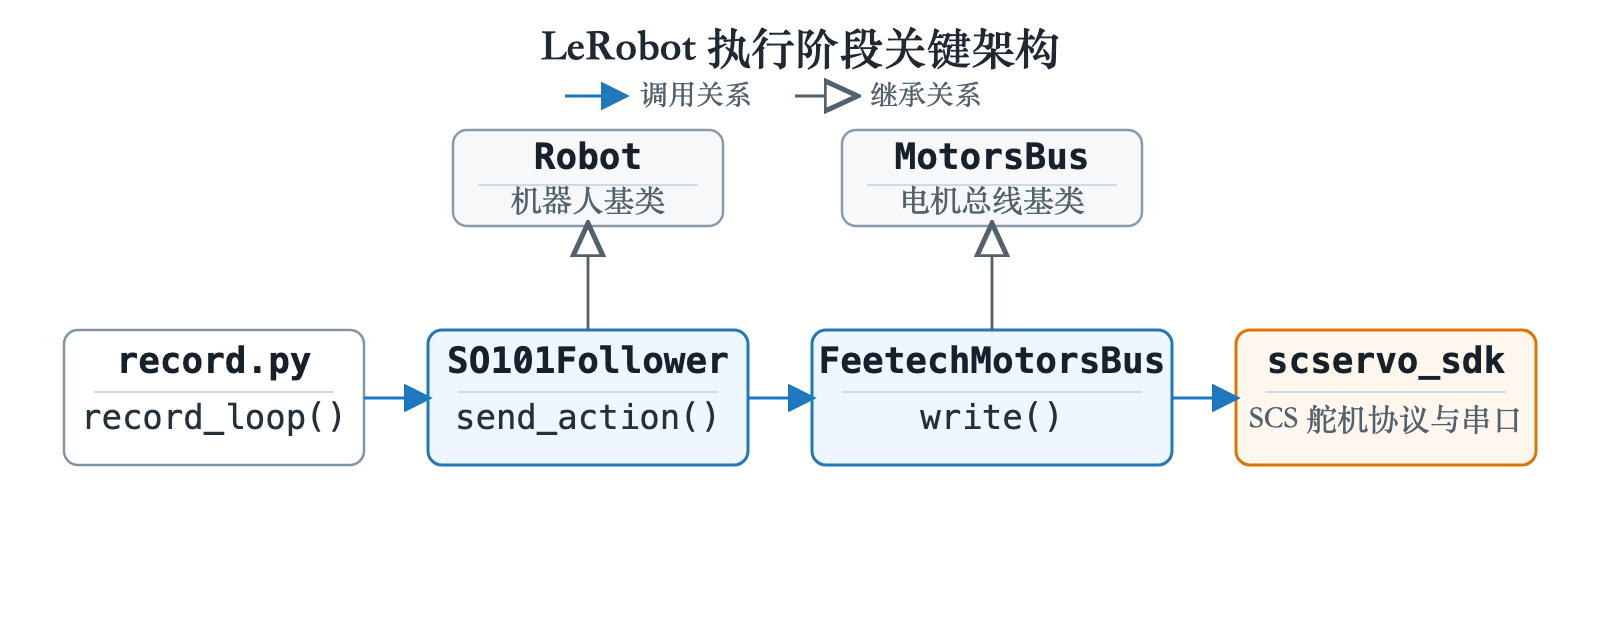
\includegraphics[width=\textwidth]{3_性能分析/image/execution_callstack_software.png}
  \caption{LeRobot 执行阶段关键类关系与调用关系}
  \label{fig:execution-callstack-software}
\end{figure}

\subsubsection{sync\_write 写链路：从电机总线到串口写入}\label{sec:sync-write-chain}

图~\ref{fig:sync-write-chain} 展示了 \texttt{send\_action()} 触发的完整写链路，
横跨五个软件层：\texttt{MotorsBus}（归一化/编码）$\to$ \texttt{GroupSyncWrite}（组包）$\to$
\texttt{GroupSyncWrite.syncWriteTxOnly()}（协议帧）$\to$ \texttt{PortHandler}（串口管理）$\to$
\texttt{ser.write()}（内核写入）。

\texttt{\_setup\_sync\_writer} 设置寄存器地址（\texttt{start\_address=42}，Goal\_Position）与数据长度（2 字节），
\texttt{addParam(id, data)} 将每个电机的目标位置序列化为 \texttt{[lo, hi]} 存入 \texttt{data\_dict[id]}；
随后 \texttt{makeParam()} 将 6 个电机数据拼成 16 字节负载，\texttt{syncWriteTxOnly()} 追加协议头与校验字节，
构造出完整的 26 字节 SYNC\_WRITE 帧（\texttt{FF FF FE 16 83 2A 02 [id lo hi] × 6 CS}），
广播 ID \texttt{0xFE} 意味着无需等待任何舵机回包；
最终 \texttt{port.writePort(pkt)} 在 \texttt{is\_using=False} 的条件下调用 \texttt{ser.write()} 将帧写入串口，
写完即返回，无 RX 阶段，随后 \texttt{clearParam()} 重置组包缓冲区。

写链路的核心特性是``发完即返回''——广播帧不要求舵机回包，Python 侧耗时约
1--3 ms，瓶颈为 USB $\to$ UART 的物理传输，而非软件开销。

\begin{figure}[htbp]
  \centering
  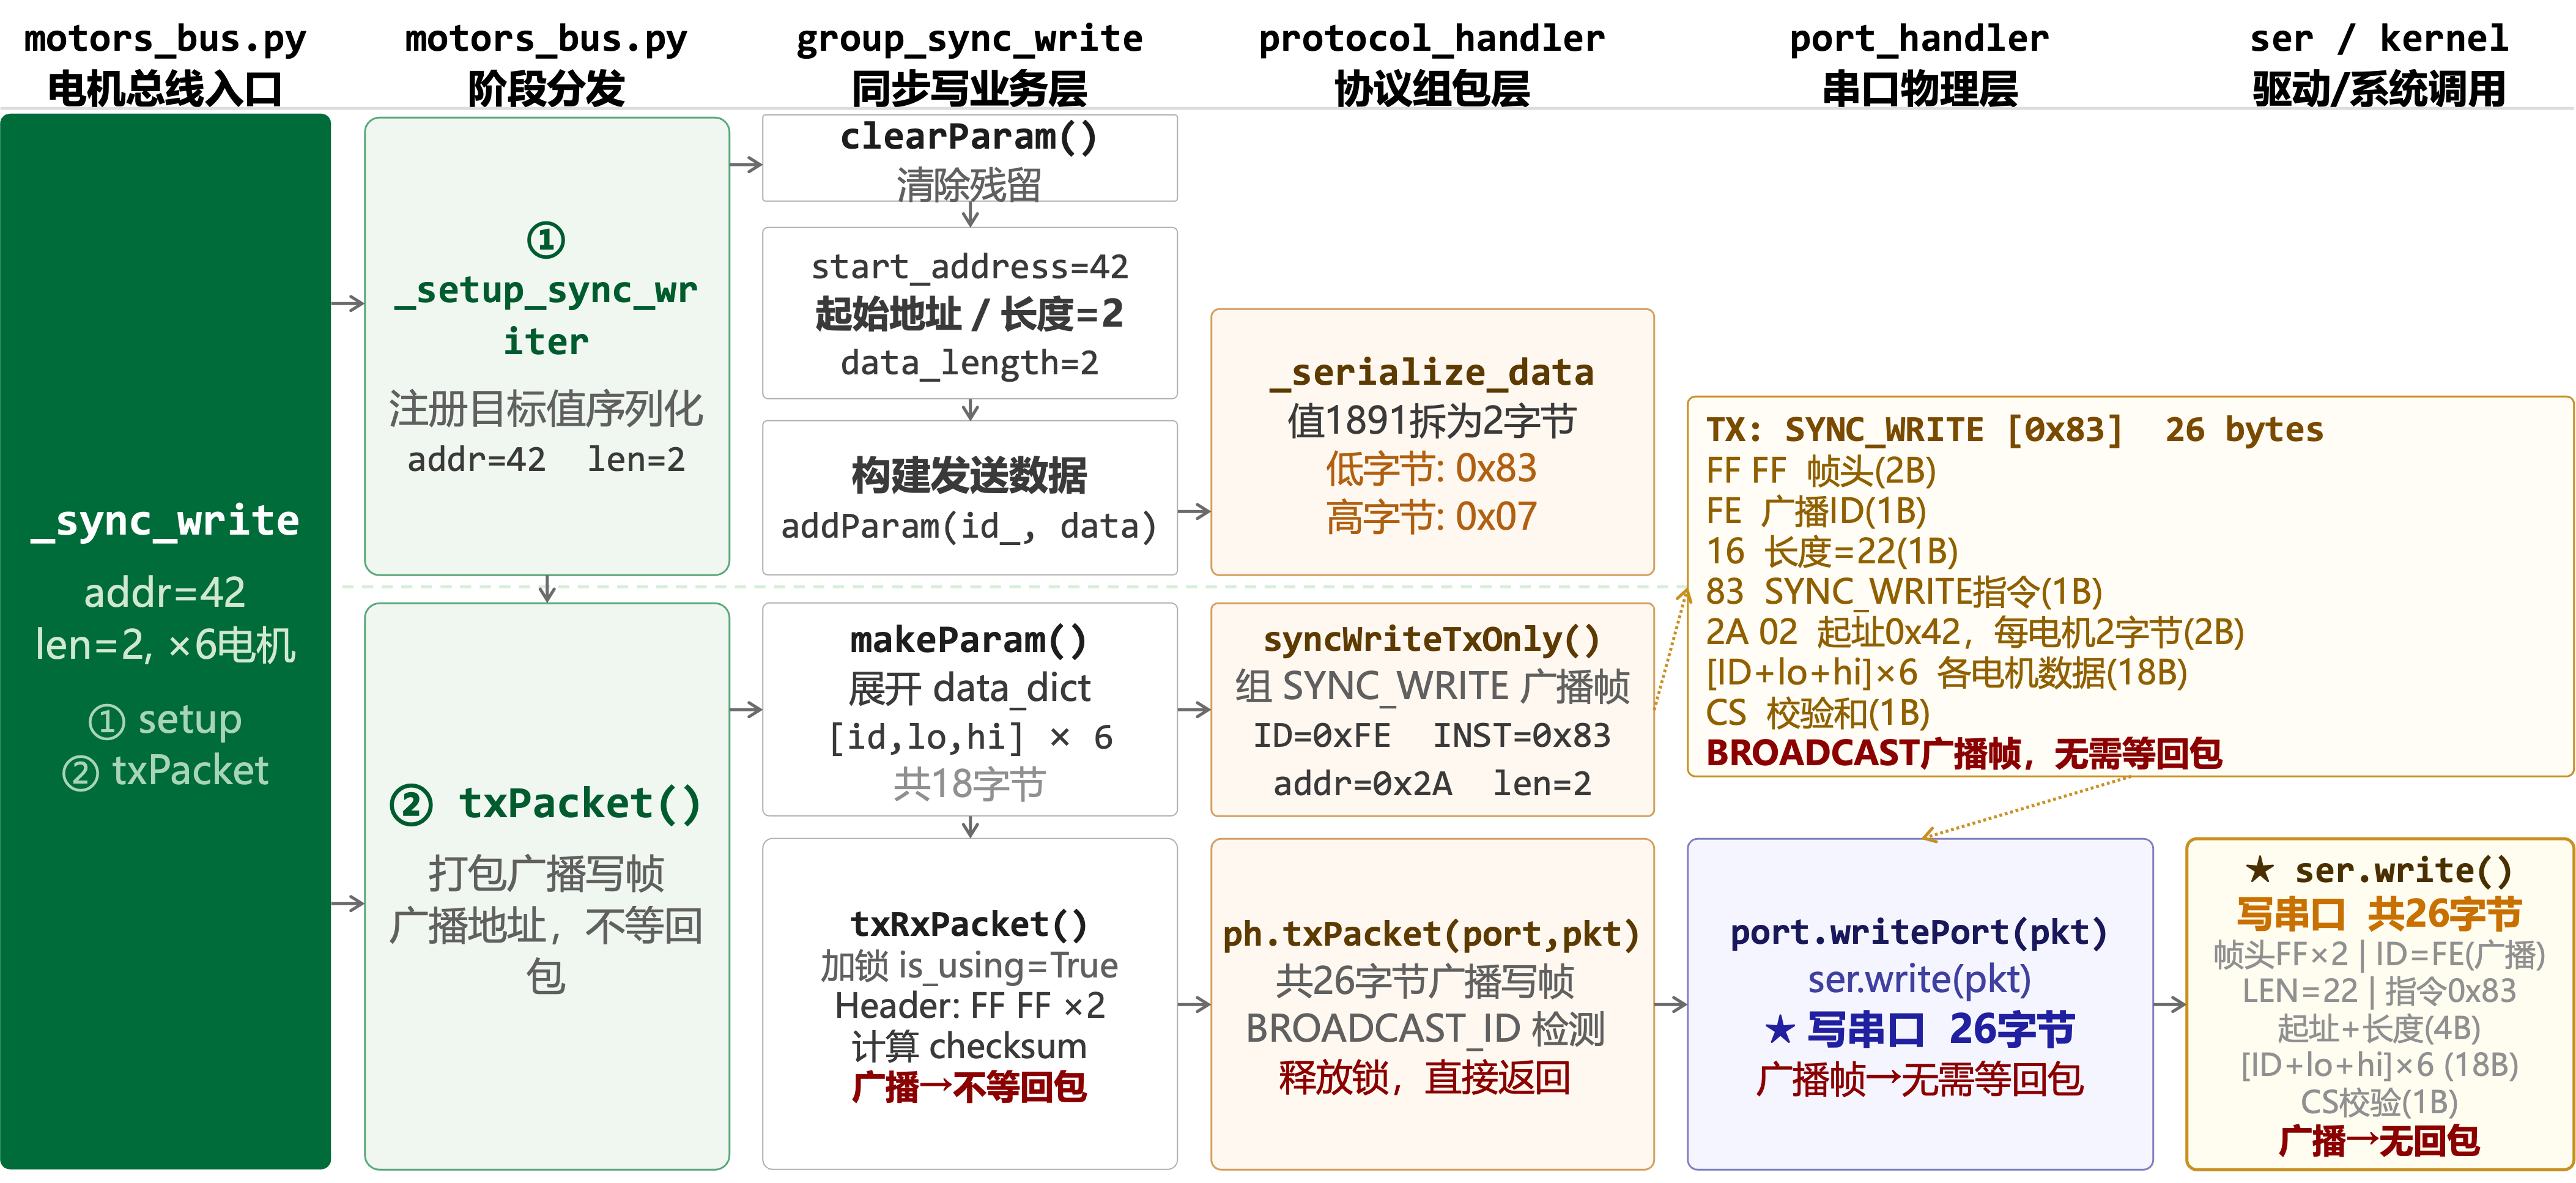
\includegraphics[width=\textwidth]{3_性能分析/image/sync_write_chain.png}
  \caption{sync\_write 写链路：motors\_bus.py $\to$ GroupSyncWrite $\to$ ProtocolHandler $\to$ PortHandler $\to$ ser.write()}
  \label{fig:sync-write-chain}
\end{figure}

\subsubsection{sync\_read 读链路：从请求帧到逐电机轮询回包}\label{sec:sync-read-chain}

图~\ref{fig:sync-read-chain} 展示了 \texttt{get\_observation()} 触发的读链路。
与写链路共享前三层软件栈，但在 \texttt{PortHandler} 层之后分叉为完整的``发送请求帧 + 逐电机轮询''双阶段。

关键数据路径如下：
\begin{enumerate}[leftmargin=2em]
  \item \textbf{请求帧发送}：\texttt{syncReadTx()} 构造 SYNC\_READ 帧
        （指令字节 \texttt{0x82}，寄存器地址 \texttt{0x38}/56，读长度 2），
        经 \texttt{ph.txPacket()} 调用 \texttt{writePort()} $\to$ \texttt{ser.write()} 写出。
        帧格式：\texttt{FF FF FE 0A 82 38 02 01 02 03 04 05 06 CS}。
  \item \textbf{逐电机回包}：\texttt{rxPacket()} 对 \texttt{data\_dict} 中每个 ID 依次调用
        \texttt{readRx(port, id, 2)}，后者调用 \texttt{ph.rxPacket(port)} $\to$ \texttt{ser.read(n)}。
        \texttt{ser.read(n)} 内部以 \texttt{while} 轮询加超时退出，等待每个电机按 ID 顺序
        在半双工总线上依次发回状态帧（\texttt{FF FF id 04 00 lo hi CS}）。
  \item \textbf{数据解析}：\texttt{getData(id, 56, 2)} 计算偏移量 \texttt{offset = 56-56 = 0}，
        取 \texttt{data[0], data[1]} 合成 16-bit 位置值（\texttt{SCS\_MAKEWORD}），
        最终返回 \texttt{\{1: 2381, …, 6: 1500\}} 形式的字典。
\end{enumerate}

读链路耗时约 1.2 ms，主要来源于 6 次串行回包等待。半双工总线在等待回包期间
不能发送任何其他指令，这是写链路无法与读链路并行化的物理根因。

\begin{figure}[htbp]
  \centering
  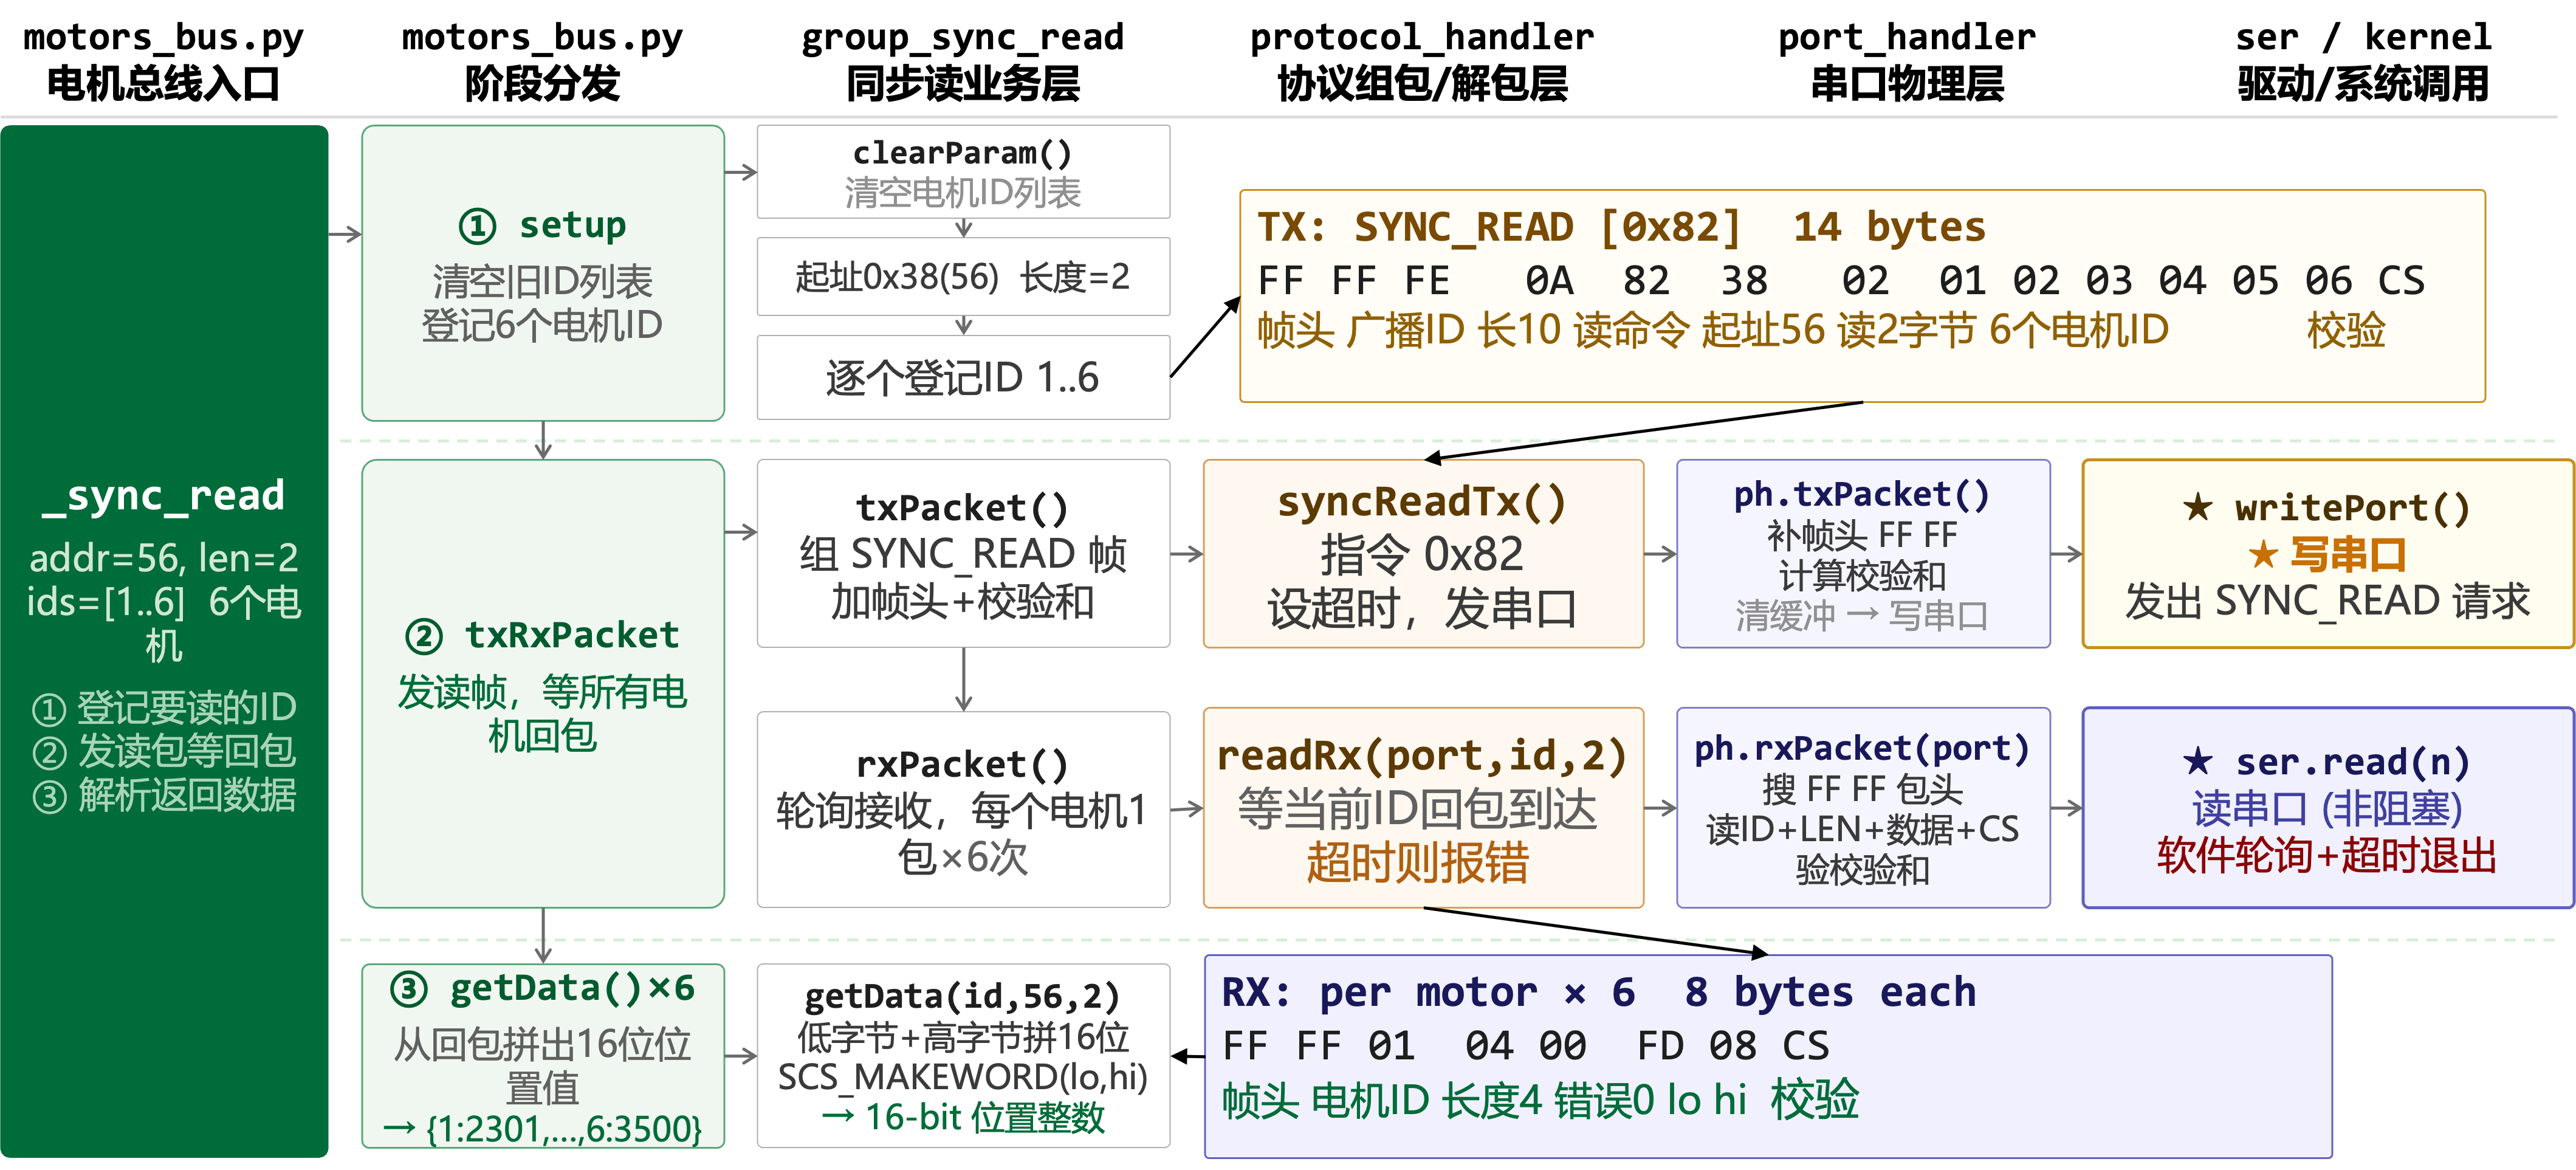
\includegraphics[width=\textwidth]{3_性能分析/image/sync_read_chain.png}
  \caption{sync\_read 读链路：motors\_bus.py $\to$ GroupSyncRead $\to$ ProtocolHandler $\to$ PortHandler $\to$ ser.read() 轮询}
  \label{fig:sync-read-chain}
\end{figure}

\textbf{关键性能结论}\label{sec:execution-conclusion}：
综合 \texttt{sync\_read} 与 \texttt{sync\_write} 两条路径可以看出，
执行阶段的主要耗时并不来自 Linux 系统调用本身。\texttt{write} 系统调用仅约
38 $\mu$s，\texttt{read} 也处于类似量级；实际观测到的 \texttt{sync\_read}
约 1.2 ms、\texttt{sync\_write} 约 1--3 ms，主要由 1 Mbps 波特率下的
SCServo 总线传输决定。具体来说，Sync Read 指令帧约 14--15 字节，
Sync Write 指令帧约 26 字节（6 ID $\times$ 4 字节位置数据，加上包头与校验），
串口物理传输时间构成耗时主体。因此，执行阶段瓶颈位于半双工舵机总线和协议物理层，
而不是 Python、SDK 封装或系统调用路径。进一步地，同一时刻总线只能容纳一个方向的传输，
若将读写简单异步并发，反而可能造成总线竞争和指令帧损坏；同时，
\texttt{send\_action()} 中 read-modify-write 的安全限幅链路依赖同步读返回的实时位置，
异步化会破坏这一控制不变量。因此，舵机读写不适合作为本文主要异步优化方向
（详见 \S\ref{sec:async-feasibility}）。

